\begin{enumerate}
\item Construct a triangle with sides 5 cm, 4 cm and 6 cm. Then construct another triangle whose sides are $\frac{2}{3}$ times the corresponding sides of first triangle.

\item In \figref{fig:fig6}, AB and CD are two diameters of a circle with centre O, which are perpendicular to each other. OB is the diameter of the smaller circle. If OA =7 cm, find the area of shaded region .$\brak{ \pi = \frac{22}{7}}$\\
	\begin{figure}[H]
		\centering
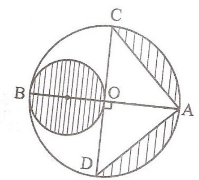
\includegraphics[width=\columnwidth]{figs/6.png}
\caption{AB and CD diameters of circle}
\label{fig:fig6}
	\end{figure}
	\end{enumerate}
